\subsection{Behandlung von verrauschten Daten (Jan)}

In der Simulation funktioniert unsere Implementierung nun sehr gut, allerdings haben wir bisher mit perfekten Laserdaten und nur Odometrierauschen getestet. Für den Umstieg auf den Roboter haben wir zunächst ein hauptsächlich lineares Rauschen auf den Laserdaten des Roboters in der Simulation eingestellt. Durch die verrauschten Laserdaten wurden die Winkel der Wände stark verzerrt und sowohl eine Korrektur der Rotation, als auch der Translation war nicht mehr sinnvoll möglich.

%TODO bild ohne rauschbehandlung, alles kaputt

Um auch mit verrauschten Laserdaten arbeiten zu können haben wir zwei Ansätze ausprobiert. Der erste Ansatz bezieht sich erstmal nur auf die Berechnung der Winkelhistogramme für die Rotationskorrektur. Wie in Kapitel~\ref{sec:winkelhistogramme} beschrieben, haben wir zu Beginn zwei aufeinanderfolgende Scanpunkte für die Berechnung der Ausrichtung der Wand genommen. Wie in Abbildung~\ref{fig:wandRauschen} (blau) zu sehen ist, kann so durch verrauschte Daten ein sehr starker Fehler entstehen. Um dieses Problem zu lösen nehmen wir nun für die Berechnung der Ausrichtung an einem Punkt i nicht die Differenz der Punkte i und i+1 sondern die Differenz der Punkte i-ANGLENOISECONST und i+ANGLENOISECONST. Als ANGLENOISECONST haben wir 10 gewählt. Wie in Abbildung~\ref{fig:wandRauschen} (grün) schematisch dargestellt ist, kann dies den Fehler stark verringern.

\begin{figure}
	\centering
	\includegraphics[width=14cm]{wandRauschen}
	\caption{Berechnung der Ausrichtung einer Wand anhand von verrauschten Scandaten. In Blau mithilfe zweier aufeinander folgenden Scanpunkten und in Grün mithilfe zweier weiter auseinanderliegenden Scanpunkten}
	\label{fig:wandRauschen}
\end{figure}

Diese Änderung führte dazu, dass die Rotationskorrektur mit verrauschten Laserdaten enorm verbessert wurde. Die daraus resultierende bessere Ausrichtung auf die Hauptachsen half auch bei der Translationskorrektur, da die Maxima der Wände aber dennoch etwas gestreut waren mussten wir auch hier noch nachbessern.

Der zweite Ansatz sollte nun auch die Translationskorrektur verbessern. Hierzu wurden die kompletten Scandaten vor der Histogrammberechnung vorverarbeitet. Die Koordinate eines jeden Scanpunkts wurde nun berechnet indem die 8 Nachbarpunkte (4 in jeder Richtung) und der Punkt selber gemittelt wurden.

Ein Test ergab, dass das beste Ergebnis erzielt wurde, wenn beide Ansätze kombiniert werden. Dabei wird der erste Ansatz auf die gemittelten Daten des zweiten Ansatzes angewendet. Eine Folge beider Ansätze ist, dass zwar die Wände gerader erscheinen, aber Ecken eher zu Kurven werden. Dies ist für die Berechnung der Rotationen und Verschiebungen aber nicht so wichtig, wie dass die Wände gerade erscheinen. In die Karte werden dann die unveränderten Scanpunkte eingetragen.